%!TEX root = ../main.tex
\chapter{Pandas --- Analyse de Donn\'ees}
\label{ch:pandas}

\begin{intuition}
Imaginez un tableur comme Excel, mais pilot\'e enti\`erement par du code Python.
C'est exactement ce que propose \textbf{Pandas}\index{Pandas} : une biblioth\`eque
puissante pour charger, explorer, filtrer et analyser des donn\'ees tabulaires.
En sciences, la majorit\'e des donn\'ees exp\'erimentales se pr\'esentent sous forme
de tableaux --- Pandas est l'outil id\'eal pour les manipuler.
\end{intuition}

% ----------------------------------------------------------------
\section{S\'eries et DataFrames}
\index{Series}\index{DataFrame}

Pandas repose sur deux structures fondamentales :

\begin{definition}[Series et DataFrame]
Une \textbf{Series} est une colonne de donn\'ees \'etiquet\'ee (comme un vecteur avec un index).
Un \textbf{DataFrame} est un tableau \`a deux dimensions compos\'e de plusieurs Series
partageant le m\^eme index.
\end{definition}

\begin{center}
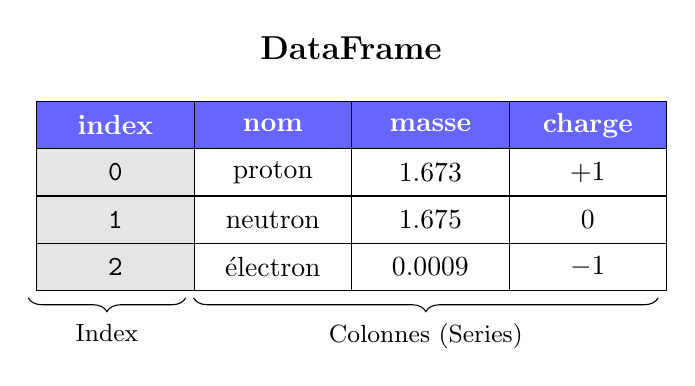
\begin{tikzpicture}[
  cell/.style={draw, minimum width=2cm, minimum height=0.6cm, anchor=north west},
  header/.style={cell, fill=blue!60, text=white, font=\bfseries},
  indexcell/.style={cell, fill=gray!20, font=\ttfamily},
]
  % Headers
  \node[header] at (0,0) {index};
  \node[header] at (2,0) {nom};
  \node[header] at (4,0) {masse};
  \node[header] at (6,0) {charge};
  % Row 0
  \node[indexcell] at (0,-0.6) {0};
  \node[cell] at (2,-0.6) {proton};
  \node[cell] at (4,-0.6) {1.673};
  \node[cell] at (6,-0.6) {+1};
  % Row 1
  \node[indexcell] at (0,-1.2) {1};
  \node[cell] at (2,-1.2) {neutron};
  \node[cell] at (4,-1.2) {1.675};
  \node[cell] at (6,-1.2) {0};
  % Row 2
  \node[indexcell] at (0,-1.8) {2};
  \node[cell] at (2,-1.8) {\'electron};
  \node[cell] at (4,-1.8) {0.0009};
  \node[cell] at (6,-1.8) {$-1$};
  % Labels
  \draw[decorate, decoration={brace, amplitude=5pt, mirror}] (-0.1,-2.5) -- (1.9,-2.5)
    node[midway, below=6pt, font=\small] {Index};
  \draw[decorate, decoration={brace, amplitude=5pt, mirror}] (2.0,-2.5) -- (7.9,-2.5)
    node[midway, below=6pt, font=\small] {Colonnes (Series)};
  \node[above, font=\large\bfseries] at (4,0.4) {DataFrame};
\end{tikzpicture}
\end{center}

\begin{codeblock}[title=\textbf{Python}]
\begin{minted}{python}
import pandas as pd

# Cr\'eer une Series
masses = pd.Series([1.673, 1.675, 0.0009],
                   index=["proton", "neutron", "electron"])
print(masses)
\end{minted}
\end{codeblock}

\begin{codeoutput}
\begin{verbatim}
proton      1.6730
neutron     1.6750
electron    0.0009
dtype: float64
\end{verbatim}
\end{codeoutput}

% ----------------------------------------------------------------
\section{Charger des donn\'ees : \py{pd.read\_csv}}
\index{read\_csv}

En pratique, on charge rarement des donn\'ees \`a la main. Pandas lit de nombreux
formats : CSV, Excel, JSON, SQL, etc. Nous utiliserons le jeu de donn\'ees
\texttt{tips}\index{tips (dataset)} disponible dans Seaborn.

\begin{codeblock}[title=\textbf{Python}]
\begin{minted}{python}
import seaborn as sns

tips = sns.load_dataset("tips")
print(type(tips))
print(tips.shape)
\end{minted}
\end{codeblock}

\begin{codeoutput}
\begin{verbatim}
<class 'pandas.core.frame.DataFrame'>
(244, 7)
\end{verbatim}
\end{codeoutput}

Le DataFrame \py{tips} contient 244 lignes (observations) et 7 colonnes.

% ----------------------------------------------------------------
\section{Exploration rapide}
\index{head}\index{info}\index{describe}\index{shape}

\begin{codeblock}[title=\textbf{Python}]
\begin{minted}{python}
# Premi`eres lignes
print(tips.head(3))
\end{minted}
\end{codeblock}

\begin{codeoutput}
\begin{verbatim}
   total_bill   tip     sex smoker  day    time  size
0       16.99  1.01  Female     No  Sun  Dinner     2
1       10.34  1.66    Male     No  Sun  Dinner     3
2       21.01  3.50    Male     No  Sun  Dinner     3
\end{verbatim}
\end{codeoutput}

\begin{codeblock}[title=\textbf{Python}]
\begin{minted}{python}
# R\'esum\'e statistique
print(tips.describe().round(2))
\end{minted}
\end{codeblock}

\begin{codeoutput}
\begin{verbatim}
       total_bill     tip    size
count      244.00  244.00  244.00
mean        19.79    3.00    2.57
std          8.90    1.38    0.95
min          3.07    1.00    1.00
25%         13.35    2.00    2.00
50%         17.80    2.90    2.00
75%         24.13    3.56    3.00
max         50.81   10.00    6.00
\end{verbatim}
\end{codeoutput}

\begin{codeblock}[title=\textbf{Python}]
\begin{minted}{python}
tips.info()
\end{minted}
\end{codeblock}

\begin{codeoutput}
\begin{verbatim}
<class 'pandas.core.frame.DataFrame'>
RangeIndex: 244 entries, 0 to 243
Data columns (total 7 columns):
 #   Column      Non-Null Count  Dtype
---  ------      --------------  -----
 0   total_bill  244 non-null    float64
 1   tip         244 non-null    float64
 2   sex         244 non-null    category
 3   smoker      244 non-null    category
 4   day         244 non-null    category
 5   time        244 non-null    category
 6   size        244 non-null    int64
\end{verbatim}
\end{codeoutput}

% ----------------------------------------------------------------
\section{S\'election de donn\'ees}
\index{loc}\index{iloc}

\begin{definition}[loc vs iloc]
\py{loc} s\'electionne par \textbf{\'etiquettes} (noms de lignes/colonnes).
\py{iloc} s\'electionne par \textbf{positions enti\`eres} (indices num\'eriques).
\end{definition}

\begin{codeblock}[title=\textbf{Python}]
\begin{minted}{python}
# S\'electionner une colonne
print(tips["total_bill"].head(3))

# S\'electionner par position (ligne 0, colonne 1)
print(tips.iloc[0, 1])      # 1.01

# S\'electionner par \'etiquette
print(tips.loc[0, "tip"])    # 1.01

# Plusieurs colonnes
subset = tips[["total_bill", "tip"]].head(3)
print(subset)
\end{minted}
\end{codeblock}

\begin{codeoutput}
\begin{verbatim}
0    16.99
1    10.34
2    21.01
Name: total_bill, dtype: float64
1.01
1.01
   total_bill   tip
0       16.99  1.01
1       10.34  1.66
2       21.01  3.50
\end{verbatim}
\end{codeoutput}

% ----------------------------------------------------------------
\section{Filtrage avec des masques bool\'eens}
\index{masque bool\'een}\index{filtrage}

\begin{codeblock}[title=\textbf{Python}]
\begin{minted}{python}
# Additions sup\'erieures `a 40 €
gros_repas = tips[tips["total_bill"] > 40]
print(gros_repas[["total_bill", "tip", "size"]])
\end{minted}
\end{codeblock}

\begin{codeoutput}
\begin{verbatim}
     total_bill   tip  size
11        35.26  5.00     4
23        39.42  7.58     4
39        31.27  5.00     3
47        32.40  6.00     4
56        38.01  3.00     1
59        48.27  6.73     4
170       50.81  10.00    3
182       45.35  3.50     3
197       43.11  5.00     4
212       48.33  9.00     4
\end{verbatim}
\end{codeoutput}

\begin{codeblock}[title=\textbf{Python}]
\begin{minted}{python}
# Conditions multiples : d\^iners du dimanche avec pourboire > 5 €
filtre = tips[(tips["day"] == "Sun") & (tips["tip"] > 5)]
print(f"Nombre de r\'esultats : {len(filtre)}")
print(filtre[["total_bill", "tip", "day"]].head())
\end{minted}
\end{codeblock}

\begin{codeoutput}
\begin{verbatim}
Nombre de resultats : 11
     total_bill    tip  day
23        39.42   7.58  Sun
39        31.27   5.00  Sun
44        30.40   5.60  Sun
47        32.40   6.00  Sun
52        34.81   5.20  Sun
\end{verbatim}
\end{codeoutput}

% ----------------------------------------------------------------
\section{Agr\'egation avec GroupBy}
\index{groupby}\index{agr\'egation}

L'op\'eration \py{groupby} permet de regrouper les donn\'ees selon une variable
cat\'egorielle, puis d'appliquer une fonction d'agr\'egation.

\begin{codeblock}[title=\textbf{Python}]
\begin{minted}{python}
# Pourboire moyen par jour
par_jour = tips.groupby("day")["tip"].mean().round(2)
print(par_jour)
\end{minted}
\end{codeblock}

\begin{codeoutput}
\begin{verbatim}
day
Thur    2.77
Fri     2.73
Sat     2.99
Sun     3.26
Name: tip, dtype: float64
\end{verbatim}
\end{codeoutput}

\begin{codeblock}[title=\textbf{Python}]
\begin{minted}{python}
# Statistiques multiples
stats = tips.groupby("sex")[["total_bill", "tip"]].agg(["mean", "std"])
print(stats.round(2))
\end{minted}
\end{codeblock}

\begin{codeoutput}
\begin{verbatim}
       total_bill        tip
             mean   std mean  std
sex
Male        20.74  9.25 3.09 1.49
Female      18.06  8.01 2.83 1.16
\end{verbatim}
\end{codeoutput}

% ----------------------------------------------------------------
\section{Visualisation rapide avec \py{df.plot()}}
\index{plot (Pandas)}

Pandas int\`egre matplotlib pour cr\'eer des graphiques en une ligne.

\begin{codeblock}[title=\textbf{Python}]
\begin{minted}{python}
import matplotlib.pyplot as plt

# Histogramme des additions
tips["total_bill"].plot(kind="hist", bins=20, edgecolor="black",
                        title="Distribution des additions")
plt.xlabel("Addition (€)")
plt.ylabel("Fr\'equence")
plt.show()

# Pourboire moyen par jour (diagramme en barres)
tips.groupby("day")["tip"].mean().plot(kind="bar", color="blue",
                                        title="Pourboire moyen par jour")
plt.ylabel("Pourboire moyen (€)")
plt.show()
\end{minted}
\end{codeblock}

\begin{codeblock}[title=\textbf{Python}]
\begin{minted}{python}
# Nuage de points : addition vs pourboire
tips.plot(kind="scatter", x="total_bill", y="tip", alpha=0.6,
          title="Pourboire en fonction de l'addition")
plt.xlabel("Addition (€)")
plt.ylabel("Pourboire (€)")
plt.show()
\end{minted}
\end{codeblock}

\begin{remarque}
Pour des visualisations plus \'elabor\'ees, on peut utiliser Seaborn ou Matplotlib
directement. La m\'ethode \py{df.plot()} est id\'eale pour une exploration rapide.
\end{remarque}

% ----------------------------------------------------------------
\section{Cr\'eer de nouvelles colonnes}

\begin{codeblock}[title=\textbf{Python}]
\begin{minted}{python}
# Calculer le pourcentage de pourboire
tips["tip_pct"] = (tips["tip"] / tips["total_bill"] * 100).round(1)
print(tips[["total_bill", "tip", "tip_pct"]].head(4))
\end{minted}
\end{codeblock}

\begin{codeoutput}
\begin{verbatim}
   total_bill   tip  tip_pct
0       16.99  1.01      5.9
1       10.34  1.66     16.1
2       21.01  3.50     16.7
3       23.68  3.31     14.0
\end{verbatim}
\end{codeoutput}

% ----------------------------------------------------------------
\begin{errmark}{Erreurs fr\'equentes avec Pandas}
\begin{enumerate}
  \item \textbf{SettingWithCopyWarning}\index{SettingWithCopyWarning} --- Quand on modifie
    une <<~tranche~>> d'un DataFrame, Pandas ne sait pas si on modifie l'original
    ou une copie. Solution : utilisez \py{.loc[]} ou \py{.copy()} explicitement.
\begin{minted}{python}
# MAUVAIS : peut d\'eclencher un warning
subset = tips[tips["day"] == "Sun"]
subset["tip_pct"] = subset["tip"] / subset["total_bill"]

# BON : copie explicite
subset = tips[tips["day"] == "Sun"].copy()
subset["tip_pct"] = subset["tip"] / subset["total_bill"]
\end{minted}
  \item \textbf{Confondre \py{loc} et \py{iloc}} --- \py{loc[1]} acc\`ede \`a la ligne
    dont l'\textbf{\'etiquette} est 1 ; \py{iloc[1]} acc\`ede \`a la \textbf{deuxi\`eme} ligne
    (position 1). Apr\`es un filtrage, les \'etiquettes ne sont plus cons\'ecutives !
  \item \textbf{Oublier les parenth\`eses dans les conditions multiples} ---
    \'Ecrivez \py{(cond1) \& (cond2)}, pas \py{cond1 \& cond2}.
\end{enumerate}
\end{errmark}

% ----------------------------------------------------------------
\begin{projet}{Analyse du dataset Tips}
\begin{enumerate}
  \item Chargez le dataset \texttt{tips} avec Seaborn.
  \item Calculez le pourboire moyen selon le moment du repas (\py{time}).
  \item D\'eterminez quel jour a le plus grand nombre de clients (somme de \py{size}).
  \item Cr\'eez une colonne \py{price\_per\_person} = \py{total\_bill / size}.
  \item Tracez un histogramme de \py{price\_per\_person} et commentez la distribution.
  \item Testez si les fumeurs laissent un pourboire diff\'erent (groupby + mean).
\end{enumerate}
\end{projet}

% ----------------------------------------------------------------
\section{Exercices}

\begin{exercice}[$\star$]
Chargez le dataset \py{sns.load\_dataset("penguins")}. Affichez les 5 premi\`eres lignes,
la forme du DataFrame et le r\'esum\'e statistique. Combien y a-t-il de valeurs manquantes
par colonne ? (Indice : \py{.isna().sum()})
\end{exercice}

\begin{exercice}[$\star$]
\`A partir du dataset \texttt{tips}, s\'electionnez toutes les lignes o\`u l'addition
d\'epasse 30\,€ et le pourboire est inf\'erieur \`a 3\,€. Combien de lignes obtient-on ?
\end{exercice}

\begin{exercice}[$\star\star$]
Utilisez \py{groupby} pour calculer la moyenne et l'\'ecart-type du pourboire
selon le sexe \emph{et} le moment du repas (groupby sur deux colonnes).
Quelle cat\'egorie laisse le pourboire moyen le plus \'elev\'e ?
\end{exercice}

\begin{exercice}[$\star\star$]
Cr\'eez une nouvelle colonne \py{tip\_category} qui vaut \py{"g\'en\'ereux"} si
\py{tip\_pct > 20}, \py{"normal"} si entre 10 et 20, et \py{"faible"} sinon.
Utilisez \py{pd.cut} ou \py{np.where}. Tracez un diagramme en barres du nombre
de repas par cat\'egorie.
\end{exercice}

\begin{exercice}[$\star\star\star$]
Chargez le dataset \py{sns.load\_dataset("planets")}. Analysez la distribution des
m\'ethodes de d\'ecouverte d'exoplan\`etes au fil des ann\'ees : groupez par
\py{method} et \py{year}, comptez les d\'ecouvertes, et tracez l'\'evolution temporelle
pour les 3 m\'ethodes les plus fr\'equentes.
\end{exercice}

% ----------------------------------------------------------------
\begin{formules}{Chapitre 8 --- Pandas : l'essentiel}
\begin{tabular}{@{}p{5cm} p{9cm}@{}}
\toprule
\textbf{Op\'eration} & \textbf{Syntaxe} \\
\midrule
Charger un CSV & \py{pd.read\_csv("fichier.csv")} \\
Premi\`eres lignes & \py{df.head(n)} \\
Dimensions & \py{df.shape} \\
R\'esum\'e statistique & \py{df.describe()} \\
S\'election colonne & \py{df["col"]} ou \py{df.col} \\
S\'election par position & \py{df.iloc[ligne, colonne]} \\
S\'election par \'etiquette & \py{df.loc[ligne, "colonne"]} \\
Filtrage & \py{df[df["col"] > valeur]} \\
Agr\'egation & \py{df.groupby("col")["val"].mean()} \\
Nouvelle colonne & \py{df["new"] = expression} \\
Graphique rapide & \py{df.plot(kind="hist")} \\
\bottomrule
\end{tabular}
\end{formules}
